


\begin{figure}[]
\centering


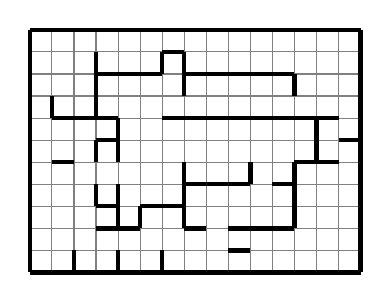
\begin{tikzpicture}[xscale=0.28, yscale=-0.28, rotate=0]
\draw[gray,thin] (0,0)--(0,11);
\draw[gray,thin] (1,0)--(1,11);
\draw[gray,thin] (2,0)--(2,11);
\draw[gray,thin] (3,0)--(3,11);
\draw[gray,thin] (4,0)--(4,11);
\draw[gray,thin] (5,0)--(5,11);
\draw[gray,thin] (6,0)--(6,11);
\draw[gray,thin] (7,0)--(7,11);
\draw[gray,thin] (8,0)--(8,11);
\draw[gray,thin] (9,0)--(9,11);
\draw[gray,thin] (10,0)--(10,11);
\draw[gray,thin] (11,0)--(11,11);
\draw[gray,thin] (12,0)--(12,11);
\draw[gray,thin] (13,0)--(13,11);
\draw[gray,thin] (14,0)--(14,11);
\draw[gray,thin] (0,0)--(15,0);
\draw[gray,thin] (0,1)--(15,1);
\draw[gray,thin] (0,2)--(15,2);
\draw[gray,thin] (0,3)--(15,3);
\draw[gray,thin] (0,4)--(15,4);
\draw[gray,thin] (0,5)--(15,5);
\draw[gray,thin] (0,6)--(15,6);
\draw[gray,thin] (0,7)--(15,7);
\draw[gray,thin] (0,8)--(15,8);
\draw[gray,thin] (0,9)--(15,9);
\draw[gray,thin] (0,10)--(15,10);
\draw[ultra thick] (6,1)--(7,1);
\draw[ultra thick] (3,1)--(3,2);
\draw[ultra thick] (3,2)--(4,2);
\draw[ultra thick] (4,2)--(5,2);
\draw[ultra thick] (6,1)--(6,2);
\draw[ultra thick] (5,2)--(6,2);
\draw[ultra thick] (7,1)--(7,2);
\draw[ultra thick] (7,2)--(8,2);
\draw[ultra thick] (8,2)--(9,2);
\draw[ultra thick] (9,2)--(10,2);
\draw[ultra thick] (10,2)--(11,2);
\draw[ultra thick] (11,2)--(12,2);
\draw[ultra thick] (3,2)--(3,3);
\draw[ultra thick] (7,2)--(7,3);
\draw[ultra thick] (12,2)--(12,3);
\draw[ultra thick] (1,3)--(1,4);
\draw[ultra thick] (1,4)--(2,4);
\draw[ultra thick] (3,3)--(3,4);
\draw[ultra thick] (2,4)--(3,4);
\draw[ultra thick] (3,4)--(4,4);
\draw[ultra thick] (6,4)--(7,4);
\draw[ultra thick] (7,4)--(8,4);
\draw[ultra thick] (8,4)--(9,4);
\draw[ultra thick] (9,4)--(10,4);
\draw[ultra thick] (10,4)--(11,4);
\draw[ultra thick] (11,4)--(12,4);
\draw[ultra thick] (12,4)--(13,4);
\draw[ultra thick] (13,4)--(14,4);
\draw[ultra thick] (4,4)--(4,5);
\draw[ultra thick] (3,5)--(4,5);
\draw[ultra thick] (13,4)--(13,5);
\draw[ultra thick] (14,5)--(15,5);
\draw[ultra thick] (1,6)--(2,6);
\draw[ultra thick] (3,5)--(3,6);
\draw[ultra thick] (4,5)--(4,6);
\draw[ultra thick] (13,5)--(13,6);
\draw[ultra thick] (12,6)--(13,6);
\draw[ultra thick] (13,6)--(14,6);
\draw[ultra thick] (7,6)--(7,7);
\draw[ultra thick] (7,7)--(8,7);
\draw[ultra thick] (8,7)--(9,7);
\draw[ultra thick] (10,6)--(10,7);
\draw[ultra thick] (9,7)--(10,7);
\draw[ultra thick] (12,6)--(12,7);
\draw[ultra thick] (11,7)--(12,7);
\draw[ultra thick] (3,7)--(3,8);
\draw[ultra thick] (4,7)--(4,8);
\draw[ultra thick] (3,8)--(4,8);
\draw[ultra thick] (5,8)--(6,8);
\draw[ultra thick] (7,7)--(7,8);
\draw[ultra thick] (6,8)--(7,8);
\draw[ultra thick] (12,7)--(12,8);
\draw[ultra thick] (4,8)--(4,9);
\draw[ultra thick] (3,9)--(4,9);
\draw[ultra thick] (5,8)--(5,9);
\draw[ultra thick] (4,9)--(5,9);
\draw[ultra thick] (7,8)--(7,9);
\draw[ultra thick] (7,9)--(8,9);
\draw[ultra thick] (9,9)--(10,9);
\draw[ultra thick] (10,9)--(11,9);
\draw[ultra thick] (12,8)--(12,9);
\draw[ultra thick] (11,9)--(12,9);
\draw[ultra thick] (9,10)--(10,10);
\draw[ultra thick] (2,10)--(2,11);
\draw[ultra thick] (4,10)--(4,11);
\draw[ultra thick] (6,10)--(6,11);
\draw[ultra thick] (0,0)--(0,11);
\draw[ultra thick] (0,0)--(15,0);
\draw[ultra thick] (15,11)--(0,11);
\draw[ultra thick] (15,11)--(15,0);
\end{tikzpicture}
\caption[An example Pentomino puzzle]{Pentomino puzzle featured on Youtube channel \emph{Cracking the Cryptic}~\protect\footnotemark}\label{fig:pentomino_puzzle1}



\end{figure}






\begin{figure}[tbp]
\hspace{1.5cm}%
\subfloat[][DAG for a 4x4 pentomino superproblem - Decomposition A]{
\centering
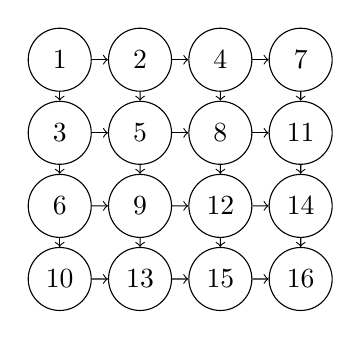
\begin{tikzpicture}[yscale=-0.91,scale=1.02]
	\node [fill=white, draw=black, shape=circle, minimum size=8mm] (1) at (0, 0) {1};
	\node [fill=white, draw=black, shape=circle, minimum size=8mm] (2) at (1, 0) {2};
	\node [fill=white, draw=black, shape=circle, minimum size=8mm] (4) at (2, 0) {4};
	\node [fill=white, draw=black, shape=circle, minimum size=8mm] (7) at (3, 0) {7};
	
	\node [fill=white, draw=black, shape=circle, minimum size=8mm] (3) at (0, 1) {3};
	\node [fill=white, draw=black, shape=circle, minimum size=8mm] (5) at (1, 1) {5};
	\node [fill=white, draw=black, shape=circle, minimum size=8mm] (8) at (2, 1) {8};
	\node [fill=white, draw=black, shape=circle, minimum size=8mm] (11) at (3, 1) {11};
	
	\node [fill=white, draw=black, shape=circle, minimum size=8mm] (6) at (0, 2) {6};
	\node [fill=white, draw=black, shape=circle, minimum size=8mm] (9) at (1, 2) {9};
	\node [fill=white, draw=black, shape=circle, minimum size=8mm] (12) at (2, 2) {12};
	\node [fill=white, draw=black, shape=circle, minimum size=8mm] (14) at (3, 2) {14};
	
	\node [fill=white, draw=black, shape=circle, minimum size=8mm] (10) at (0, 3) {10};
	\node [fill=white, draw=black, shape=circle, minimum size=8mm] (13) at (1, 3) {13};
	\node [fill=white, draw=black, shape=circle, minimum size=8mm] (15) at (2, 3) {15};
	\node [fill=white, draw=black, shape=circle, minimum size=8mm] (16) at (3, 3) {16};
	
	\draw [fill=none, ->] (1) to (3);
	\draw [fill=none, ->] (2) to (5);
	\draw [fill=none, ->] (4) to (8);
	\draw [fill=none, ->] (7) to (11);
	
	\draw [fill=none, ->] (3) to (6);
	\draw [fill=none, ->] (5) to (9);
	\draw [fill=none, ->] (8) to (12);
	\draw [fill=none, ->] (11) to (14);
	
	\draw [fill=none, ->] (6) to (10);
	\draw [fill=none, ->] (9) to (13);
	\draw [fill=none, ->] (12) to (15);
	\draw [fill=none, ->] (14) to (16);
	
	\draw [fill=none, ->] (1) to (2);
	\draw [fill=none, ->] (2) to (4);
	\draw [fill=none, ->] (4) to (7);
	
	\draw [fill=none, ->] (3) to (5);
	\draw [fill=none, ->] (5) to (8);
	\draw [fill=none, ->] (8) to (11);
	
	\draw [fill=none, ->] (6) to (9);
	\draw [fill=none, ->] (9) to (12);
	\draw [fill=none, ->] (12) to (14);
	
	\draw [fill=none, ->] (10) to (13);
	\draw [fill=none, ->] (13) to (15);
	\draw [fill=none, ->] (15) to (16);
\end{tikzpicture}
\label{fig:dag_example1215}
}\hspace{1.5cm}%
\subfloat[18cm][DAG for a 4x4 pentomino superproblem - Decomposition B]{
\centering
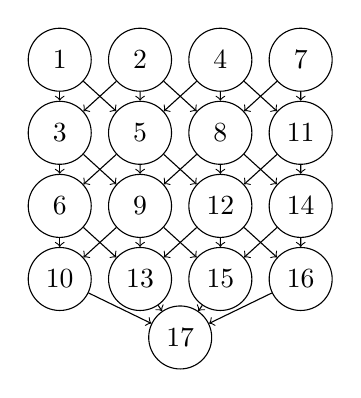
\begin{tikzpicture}[yscale=-0.91,scale=1.02]
	\node [fill=white, draw=black, shape=circle, minimum size=8mm] (1) at (0, 0) {1};
	\node [fill=white, draw=black, shape=circle, minimum size=8mm] (2) at (1, 0) {2};
	\node [fill=white, draw=black, shape=circle, minimum size=8mm] (4) at (2, 0) {4};
	\node [fill=white, draw=black, shape=circle, minimum size=8mm] (7) at (3, 0) {7};
	
	\node [fill=white, draw=black, shape=circle, minimum size=8mm] (3) at (0, 1) {3};
	\node [fill=white, draw=black, shape=circle, minimum size=8mm] (5) at (1, 1) {5};
	\node [fill=white, draw=black, shape=circle, minimum size=8mm] (8) at (2, 1) {8};
	\node [fill=white, draw=black, shape=circle, minimum size=8mm] (11) at (3, 1) {11};
	
	\node [fill=white, draw=black, shape=circle, minimum size=8mm] (6) at (0, 2) {6};
	\node [fill=white, draw=black, shape=circle, minimum size=8mm] (9) at (1, 2) {9};
	\node [fill=white, draw=black, shape=circle, minimum size=8mm] (12) at (2, 2) {12};
	\node [fill=white, draw=black, shape=circle, minimum size=8mm] (14) at (3, 2) {14};
	
	\node [fill=white, draw=black, shape=circle, minimum size=8mm] (10) at (0, 3) {10};
	\node [fill=white, draw=black, shape=circle, minimum size=8mm] (13) at (1, 3) {13};
	\node [fill=white, draw=black, shape=circle, minimum size=8mm] (15) at (2, 3) {15};
	\node [fill=white, draw=black, shape=circle, minimum size=8mm] (16) at (3, 3) {16};
	
	\node [fill=white, draw=black, shape=circle, minimum size=8mm] (17) at (1.5, 3.8) {17};
	
	\draw [fill=none, ->] (1) to (3);
	\draw [fill=none, ->] (2) to (5);
	\draw [fill=none, ->] (4) to (8);
	\draw [fill=none, ->] (7) to (11);
	
	\draw [fill=none, ->] (3) to (6);
	\draw [fill=none, ->] (5) to (9);
	\draw [fill=none, ->] (8) to (12);
	\draw [fill=none, ->] (11) to (14);
	
	\draw [fill=none, ->] (6) to (10);
	\draw [fill=none, ->] (9) to (13);
	\draw [fill=none, ->] (12) to (15);
	\draw [fill=none, ->] (14) to (16);
	
	\draw [fill=none, ->] (1) to (5);
	\draw [fill=none, ->] (2) to (8);
	\draw [fill=none, ->] (4) to (11);
	
	\draw [fill=none, ->] (3) to (9);
	\draw [fill=none, ->] (5) to (12);
	\draw [fill=none, ->] (8) to (14);
	
	\draw [fill=none, ->] (6) to (13);
	\draw [fill=none, ->] (9) to (15);
	\draw [fill=none, ->] (12) to (16);
	
	\draw [fill=none, ->] (2) to (3);
	\draw [fill=none, ->] (4) to (5);
	\draw [fill=none, ->] (7) to (8);
	
	\draw [fill=none, ->] (5) to (6);
	\draw [fill=none, ->] (8) to (9);
	\draw [fill=none, ->] (11) to (12);
	
	\draw [fill=none, ->] (9) to (10);
	\draw [fill=none, ->] (12) to (13);
	\draw [fill=none, ->] (14) to (15);
	
	\draw [fill=none, ->] (10) to (17);
	\draw [fill=none, ->] (13) to (17);
	\draw [fill=none, ->] (15) to (17);
	\draw [fill=none, ->] (16) to (17);
\end{tikzpicture}
\label{fig:dag_example1216}
}




\caption[Two possible DAG arrangements for Pentomino problems]{Two DAG arrangements for solving a cascaded grid of connected sub-problems}\label{fig:pentominos_subfigure}
\end{figure}








\footnotetext{\url{youtube.com/watch?v=S2aN-s3hG6Y}}
